\section{Switch between Guardian and Citizen Mode}

\begin{figure}[h]
    \centering
    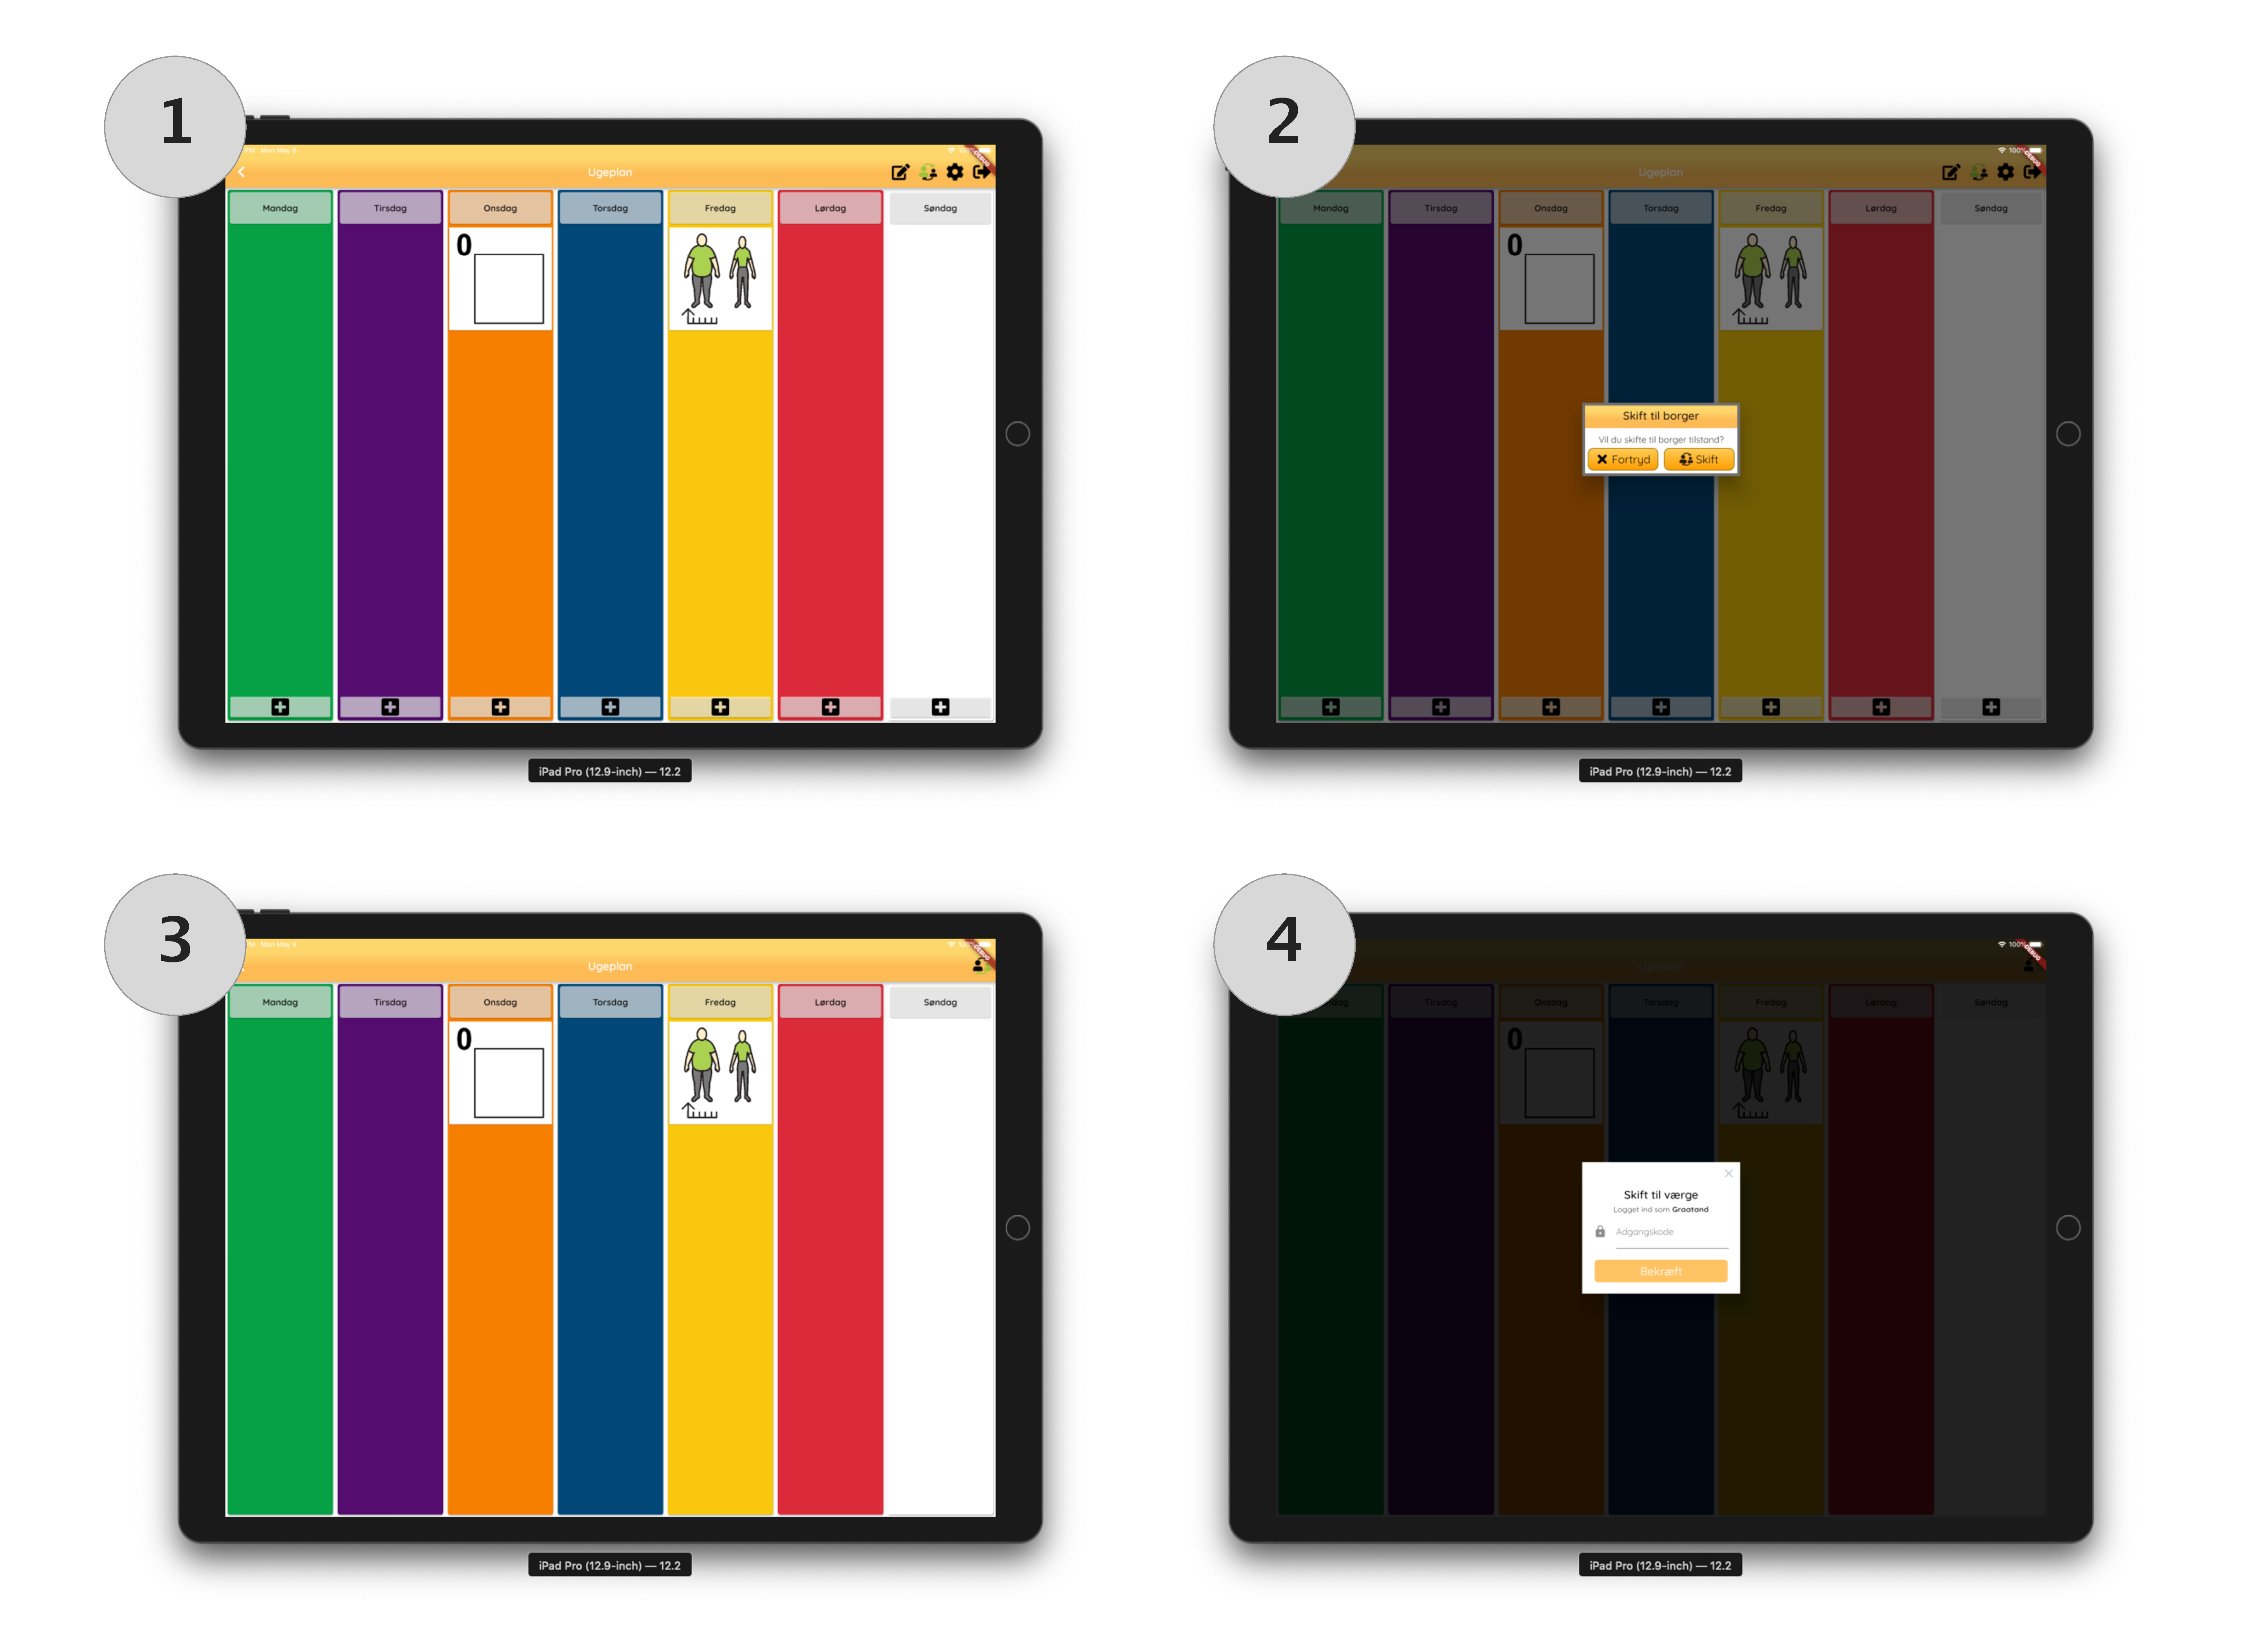
\includegraphics[width=0.8\textwidth]{figures/feature_132.pdf}
    \caption{An illustration of the final result after implementing feature 132}
    \label{fig:feature132}
\end{figure}

The feature was described as "As a user, I would like to be able to switch between guardian and citizen mode so that I can only access the parts of the system that I should be able to." Alongside the description \gls{PO} had set two requirements:

\begin{itemize}
  \item The system stores whether the user is currently in citizen or guardian mode
  \item A guardian can see the \textit{add new activities} function, but a citizen cannot
\end{itemize}

We started by adding a stream to the week-plan \gls{bloc} which sends information about whether the current mode is citizen or guardian mode. We used the stream in a \textit{StreamBuilder} in the week-plan screen, and made the visibility of the \textit{add new activity} button dependent on the state emitted from the stream.

We added a button to the application bar, which showed a \textit{change to citizen} icon when in guardian mode, and a \textit{change to guardian} icon otherwise. The user can change mode by clicking the button.

There was already implemented a dialog box asking for a password which appeared when clicking the \textit{change to guardian} icon. The user-story had no mention of a confirmation dialog box when changing to citizen mode, but we thought it would be an improvement to the application, so we implemented it after asking for permission from \gls{PO}.

During the development of the feature, we became aware of additional mode dependent functionality in other screens than the week-plan screen.  We moved the responsibility of the mode stream to the authentication \gls{bloc} to accommodate the functionalities, which makes it possible to get mode on all screens, and made no difference in how we used the mode.

The mode stream allows developers to use a \textit{StreamBuilder} widget on any screen of the application, and use conditional statements to handle functionality for the citizen and guardian mode, which offers a clean and comprehensive way to handle the restrictions.

The development of the feature was ongoing for most of the sprint, and the feature finished too late to get into the Sprint 3 release, which was because three other user stories blocked the development, as we could not finish the user story before features like the \textit{new activities} button were available.
